\section{Experimental Setup}

\begin{frame}{Dataset}

\begin{block}{}
	We use daily time series of streamflow contributions recorded from 23 Colombian reservoirs. The dataset contains 4,442 i.i.d. samples, with \(N=3,554\) used for training and \(N_*=888\) for testing.
\end{block}

\begin{figure}
	\centering
	\def\TrainEnd{1000}   % split index (x where test starts)
	\def\XMax{1500}       % max x (length of the series)
	
	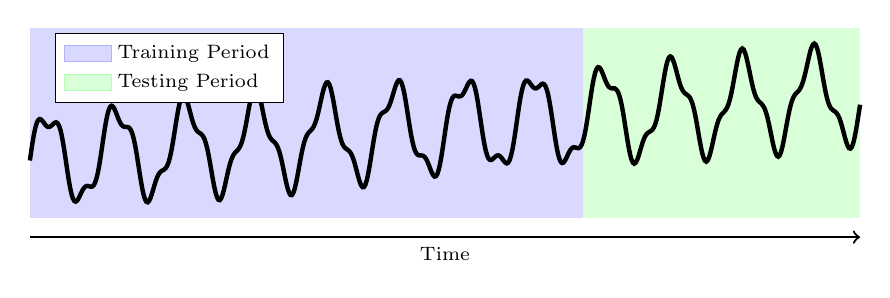
\begin{tikzpicture}
		\begin{axis}[
			font=\scriptsize,
			width=\textwidth, height=4cm,
			xmin=0, xmax=\XMax,
			axis y line=none,
			axis x line=none,
			xtick=\empty, ytick=\empty,
			grid=none,
			legend cell align=left,
			legend pos=north west,
			clip=false % allow arrow/text outside the plot area
			]
			
			% ---- shaded areas ----
			\path[fill=blue!15]  (rel axis cs:0,0) rectangle (rel axis cs:{\TrainEnd/\XMax},1);
			\path[fill=green!15] (rel axis cs:{\TrainEnd/\XMax},0) rectangle (rel axis cs:1,1);
			
			% ---- example time series (no legend entry) ----
			\addplot[ultra thick, color=black, domain=0:\XMax, samples=600, forget plot]
			{30*sin(deg(x/20)) + 8*sin(deg(x/7)) + 0.03*(x-0.6*\XMax)};
			
			% ---- legend: only shaded areas ----
			\addlegendimage{area legend, fill=blue!15, draw=blue!30}
			\addlegendentry{Training Period}
			\addlegendimage{area legend, fill=green!15, draw=green!30}
			\addlegendentry{Testing Period}
			
			% ---- time direction (arrow + label) ----
			\draw[->, thick] (rel axis cs:0,-0.10) -- (rel axis cs:1,-0.10)
			node[pos=0.5, below] {Time};
			
		\end{axis}
	\end{tikzpicture}
\end{figure}


\begin{block}{}
	The testing dataset \(\mathcal{D}_* = \{\boldsymbol{x}_{*n}, \boldsymbol{y}_{*n}\}_{n=1}^{N_*} \), where \( \boldsymbol{y}_{*n} = [y_{*n,1}, \cdots, y_{*n, D}]^\top \), collects all tasks observations at every test input \( y_{*n,d}\).
\end{block}
	
\end{frame}

\begin{frame}{Model Setup}

\begin{block}{}
	The forecasting methodology constructs the covariance function using the squared exponential kernel, facilitating smooth data mapping.
\end{block}


\[
	k_{q}\left(\boldsymbol{x}, \boldsymbol{x}' \right) = \exp\left(-\frac{1}{2}(\boldsymbol{x} - \boldsymbol{x}')^\top \boldsymbol{\Phi}_q^{-2} (\boldsymbol{x} - \boldsymbol{x}')\right)
\]

\begin{block}{}
\( \boldsymbol{\Phi}_q=\text{diag}\{\Delta_{ql}\}_{l=1}^{L} \in \mathbb{R}^{++L \times L} \) contains the length-scales. Regarding the likelihood,
\end{block}

\[
	p(\boldsymbol{Y} \mid \boldsymbol{\theta}(\boldsymbol{X})) = \prod_{n=1}^{N}\prod_{d=1}^{D} \mathcal{N}\left(y_{nd} \mid h_{d,1}(f_{d,1}(\mathbf{x}_n)), h_{d,2}(f_{d,2}(\mathbf{x}_n)) \right),
\]

\begin{block}{}
$h_{d,1}(\cdot)$ is the identity function. The baseline model is the standard LMC GP with $h_{d,2}(\cdot)$ as a constant, while the proposed model is the Chained LMC GP with $h_{d,2}(\cdot) = \ln(\exp(\cdot)+1)$.
\end{block}

\end{frame}


\begin{frame}{Performance Metrics}

\begin{block}{}
	Given the predictive mean \( \hat{\mu}_{n,d}\) and variance \( \hat{\sigma}^2_{n,d}\), the Mean Squared Error (MSE) takes the following form
\end{block}

\[
	\text{MSE} = \frac{1}{N_{*}D} \sum_{n=1}^{N_*} \sum_{d=1}^{D} \left( y_{*n,d} - \hat{\mu}_{n,d} \right)^2.
\]

\begin{block}{}
The Mean Standardized Log Loss (MSLL) \textcolor{BrandTeal}{\textbf{assesses probabilistic prediction quality}}~\cite{RasmussenW06}
\end{block}

\[
	\text{MSLL} = \frac{1}{2N_{*}D} \sum_{n=1}^{N_*} \sum_{d=1}^{D}  \frac{(y_{*n,d} - \hat{\mu}_{n,d} )^2}{\hat{\sigma}^2_{n,d}}
	- \frac{(y_{*n,d} - \mu_d)^2}{\sigma_d^2} + \ln \left(\frac{\hat{\sigma}^2_{n,d}}{\sigma_d^2}\right)
\]

\begin{block}{}
	where \( \mu_d = \frac{1}{N_*} \sum_{n=1}^{N_*} y_{*n,d}\) and \( \sigma_d^2 = \frac{1}{N_* - 1} \sum_{n=1}^{N_*} (\mu_d - y_{*n,d})^2 \).
\end{block}

\end{frame}

\begin{frame}{Hyperparameter Tuning}
	
	\begin{block}{}	
		A grid search on the baseline model fixed \(T=1\) and \(M=64\). We varied \( Q \in \{1, \cdots ,46\} \).
	\end{block}
	
	\begin{figure}[htbp]
		\centering
		\begin{tikzpicture}[font=\scriptsize]
			\begin{groupplot}[
				group style={
					group size=2 by 1,
					horizontal sep=1.5cm,
					vertical sep=1.5cm,
					xlabels at=edge bottom,
					ylabels at=edge left
				},
				width=0.5\linewidth,
				height=0.32\linewidth,
				xlabel={Number of independent GPs ($Q$)},
				ylabel={MSE},
				grid=both,
				major grid style={line width=.5pt, draw=gray!30},
				minor grid style={line width=.3pt, draw=gray!15},
				tick style={black, thick},
				axis x line=bottom,
				axis y line=left,
				xtick pos=bottom,
				ytick pos=left,
				tick align=outside,
				legend style={
					at={(rel axis cs:0.98,0.98)},
					anchor=north east,
					legend columns=2,
					/tikz/every even column/.append style={column sep=1em},
					inner sep=2pt,
					font=\scriptsize,
					nodes={scale=0.9, transform shape},
					draw=black!25,
					fill=white,
					fill opacity=0.85,
					legend cell align=left
				},
				clip=false
				]
				\nextgroupplot[
				% %xticklabels={},
				% after end axis/.code={
					% 	\node at (rel axis cs:0.5,-0.18) {(a) MSE};
					% }
				]
				% This file was created with tikzplotlib v0.10.1.
%\begin{tikzpicture}

\definecolor{darkgray176}{RGB}{176,176,176}
\definecolor{steelblue31119180}{RGB}{31,119,180}

%\begin{axis}[
%font=\tiny,
%width=\figurewidth,
%height=\figureheight,
%axis background/.style={fill=background_color},
%axis line style={white},
%tick align=inside,
%tick pos=left,
%x grid style={white},
%y grid style={white},
%xmajorgrids,
%ymajorgrids,
%xmin=-1.25, xmax=48.25,
%xtick style={color=black},
%ymajorgrids,
%ymin=0.00432172839722227, ymax=0.0132074497620714,
%ytick style={color=black}
%]
\addplot [semithick, steelblue31119180, mark=*, mark size=1, mark options={solid}]
table {%
1 0.0128035533363964
2 0.00905686675869738
3 0.00827670369639854
4 0.00647312454537253
5 0.0059998944618926
6 0.00624419146120023
7 0.00579712581238592
8 0.00571172094861466
9 0.00533441391077178
10 0.00531633238994604
11 0.00532343324902325
12 0.0050867372520667
13 0.00526346840550523
14 0.00508599694700343
15 0.00518337894714425
16 0.00513812905102857
17 0.00682742467122673
18 0.00510528673403877
19 0.00563946517817211
20 0.00551913123809022
21 0.00494528640998287
22 0.00585845931386892
23 0.00547909049889633
24 0.00472562482289723
25 0.00615358787709803
26 0.00483592747529357
27 0.0075631880355845
28 0.0056618067323409
29 0.00482810431270197
30 0.00603131705475209
31 0.00655705532258234
32 0.00710549067844106
33 0.00569378426511534
34 0.00603826998078558
35 0.00708460267778661
36 0.00849317978089477
37 0.00740070646203432
38 0.00816300146172802
39 0.00638476700981259
40 0.00632862480530453
41 0.00700173319188677
42 0.00642937589842245
43 0.00635723590641261
44 0.00655464545991826
45 0.00670091040125378
46 0.00706706114782923
};
%\end{axis}

%\end{tikzpicture}

				\nextgroupplot[
				%xticklabels={},
				ylabel={MSLL},
				xlabel={Number of independent GPs ($Q$})
				% after end axis/.code={
					% 	\node at (rel axis cs:0.5,-0.18) {(b) };
					% }
				]
				% This file was created with tikzplotlib v0.10.1.
\begin{tikzpicture}

\definecolor{darkgray176}{RGB}{176,176,176}
\definecolor{steelblue31119180}{RGB}{31,119,180}

\begin{axis}[
font=\tiny,
width=\figurewidth,
height=\figureheight,
axis background/.style={fill=background_color},
axis line style={white},
tick align=inside,
tick pos=left,
x grid style={white},
y grid style={white},
xmajorgrids,
ymajorgrids,
xmin=-1.25, xmax=48.25,
xtick style={color=black},
ymin=-0.981574217818357, ymax=-0.254980175714052,
ytick style={color=black},
%xlabel={Number of Independent GPs (Q)}
]
\addplot [semithick, steelblue31119180, mark=*, mark size=1, mark options={solid}]
table {%
1 -0.288007177627884
2 -0.486433875918135
3 -0.593083030305358
4 -0.689721765965117
5 -0.707669865514075
6 -0.720422487612926
7 -0.737789583039415
8 -0.76977958126218
9 -0.790749444413204
10 -0.801765978552222
11 -0.819791223747015
12 -0.86272547623958
13 -0.857831565839939
14 -0.876741782841828
15 -0.906781806077751
16 -0.866509321979023
17 -0.567252287936316
18 -0.918594583955142
19 -0.756984658169378
20 -0.760631883882401
21 -0.89582623985992
22 -0.717113890413948
23 -0.80039183605464
24 -0.948547215904525
25 -0.636946438064492
26 -0.942583598637442
27 -0.571591759252111
28 -0.681619424160601
29 -0.912816354860318
30 -0.626429497657631
31 -0.646795260122204
32 -0.571941714185512
33 -0.706618646926849
34 -0.619101344506579
35 -0.456559364448254
36 -0.395685084563509
37 -0.427008525048951
38 -0.399195477809696
39 -0.503866482905641
40 -0.471543594639428
41 -0.501112946719914
42 -0.473864288674822
43 -0.496469966822398
44 -0.535960786269092
45 -0.402501473063068
46 -0.518758524526979
};
\end{axis}

\end{tikzpicture}

				
			\end{groupplot}
		\end{tikzpicture}
	\end{figure}
	
	\begin{block}{}
		The MSE and MSLL decrease until \(Q=15\). Beyond this threshold, the trend becomes unstable, likely due to the increased model complexity.
	\end{block}
	
\end{frame}